\documentclass[12pt,a4paper,oneside]{book}
\usepackage[utf8]{inputenc}
\usepackage{amsmath}
\usepackage{amsfonts}
\usepackage{amssymb}
\usepackage{graphicx}
\usepackage[hidelinks]{hyperref}
\usepackage{minted}
\usepackage{tcolorbox}
\usepackage{geometry}
\usepackage{fancyhdr}
\usepackage{titlesec}
\usepackage{xcolor}
\usepackage{enumitem}
\usepackage{tikz}
\usetikzlibrary{shapes.geometric, arrows.meta, positioning}

% Setup page geometry
\geometry{
    a4paper,
    left=25mm,
    right=25mm,
    top=25mm,
    bottom=25mm
}

% Setup colors
\definecolor{primary}{RGB}{41, 128, 185}
\definecolor{secondary}{RGB}{142, 68, 173}
\definecolor{darkgray}{RGB}{50, 50, 50}

\setlength{\headheight}{14.5pt}

% Header and Footer
\pagestyle{fancy}
\fancyhf{}
\fancyhead[L]{\textcolor{primary}{\textbf{GenAI Engineering Handbook}}}
\fancyhead[R]{\thepage}
\renewcommand{\headrulewidth}{0.4pt}
\renewcommand{\footrulewidth}{0.4pt}

% Title formats
\titleformat{\chapter}[display]
  {\normalfont\huge\bfseries\color{primary}}{\chaptertitlename\ \thechapter}{20pt}{\Huge}
\titleformat{\section}
  {\normalfont\Large\bfseries\color{secondary}}{\thesection}{1em}{}
\titleformat{\subsection}
  {\normalfont\large\bfseries\color{darkgray}}{\thesubsection}{1em}{}

% Custom boxes
\newtcolorbox{infobox}[1][]{colback=blue!5!white,colframe=blue!75!black,fonttitle=\bfseries,title=#1}
\newtcolorbox{warningbox}[1][]{colback=red!5!white,colframe=red!75!black,fonttitle=\bfseries,title=#1}
\newtcolorbox{bestpractice}[1][]{colback=green!5!white,colframe=green!75!black,fonttitle=\bfseries,title=#1}

\title{\Huge \textbf{Generative AI Engineering Handbook} \\ \vspace{0.5cm} \Large The Definitive Guide for Production Systems \\ \vspace{0.2cm} \small (Comprehensive Course Notes \& Study Material)}
\author{Synthesized from Scaler Academy (L1 - L13)}
\date{\today}

\begin{document}

\maketitle
\tableofcontents
\newpage

\chapter{Foundations of Generative AI}

\section{Transformers \& Next-Token Prediction}
Generative AI relies heavily on the \textbf{Transformer architecture}. At its core, a Large Language Model's (LLM) primary objective is simply to predict the next token based on a sequence of preceding tokens.
\begin{itemize}
    \item \textbf{Tokenization:} Text is converted into smaller chunks called tokens. A rule of thumb is that 1 token is approximately 0.75 words.
    \item \textbf{Embeddings:} Tokens are mapped to high-dimensional continuous vectors. This mathematical representation captures the deep semantic meaning of words.
    \item \textbf{Self-Attention:} The core mechanism of a Transformer. It allows the model to weigh the importance of all different words in a sentence relative to a specific word, capturing immense contextual relationships.
\end{itemize}

\begin{infobox}[Core Concept: Statelessness]
LLMs are inherently stateless. Every time you make an API call to an LLM, you must provide the complete context (system prompt, user history, and new prompt). The model itself does not "remember" your past API calls. Memory is entirely an application-layer construct.
\end{infobox}

\section{Prompt Engineering \& Model Parameters}
Prompting is the interface to the model. Effective prompting aligns the model's outputs with your specific business logic.

\subsection{Hyperparameters}
\begin{itemize}
    \item \textbf{Temperature:} Controls the randomness of the model's output. A temperature of 0 makes the model strictly deterministic (always picking the highest probability token), ideal for coding and factual Q\&A. A temperature near 1 introduces creativity, ideal for creative writing.
    \item \textbf{Top-p / Top-k:} Sampling techniques that truncate the distribution of possible next tokens, forcing the model to only select from the most likely subsets.
\end{itemize}

\subsection{Prompting Strategies}
\begin{itemize}
    \item \textbf{Zero-Shot Prompting:} Asking the model to perform a task without providing any examples.
    \item \textbf{Few-Shot Prompting:} Providing 2-3 examples of desired input-output pairs to guide the structural format of the generation.
    \item \textbf{Chain of Thought (CoT):} Encouraging the model to break down complex reasoning steps by adding phrases like "Let's think step by step." This explicitly forces the model to output its intermediate reasoning tokens, vastly improving logical accuracy.
\end{itemize}

\chapter[Retrieval-Augmented Generation]{Retrieval-Augmented\\Generation (RAG)}
RAG bridges the gap between the frozen, parametric knowledge of an LLM and your real-time or private proprietary data, effectively eliminating factual hallucinations for domain-specific queries.

\section{Vector Databases \& Semantic Search}
Unlike keyword-based search (BM25), which relies on exact string matches, vector databases (like \textbf{Qdrant}, \textbf{Milvus}, or \textbf{Pinecone}) perform similarity searches on embeddings.
\begin{itemize}
    \item \textbf{Chunking \& Overlap:} Documents are too large to fit in an LLM context window. They are split into chunks (e.g., 512 tokens). An \textit{overlap} (e.g., 50 tokens) is maintained to ensure that sentences cut in half do not lose their semantic context.
    \item \textbf{Indexing:} Embeddings of these chunks are stored in a Vector DB.
    \item \textbf{Retrieval:} A user query is converted into an embedding, and the DB returns the Top-K most similar chunks using distance metrics like \textbf{Cosine Similarity} or \textbf{Euclidean Distance}.
\end{itemize}

\section{Advanced Retrieval Strategies}
Naive RAG fails with ambiguous queries or noisy documents. Production RAG implements multiple defensive strategies:
\begin{itemize}
    \item \textbf{Query Rewriting (CRAG):} Raw queries often contain pronouns ("What is its impact?"). Before querying the DB, a fast, cheap SLM rewrites the query into a standalone sentence ("What is the impact of Next.js 14 server actions?").
    \item \textbf{Hybrid Search:} Combining traditional BM25 keyword search with Dense Vector search to ensure both exact keyword hits (IDs, names) and semantic hits are retrieved.
    \item \textbf{Cross-Encoder Re-Ranking:} Vector search is fast but coarse. We retrieve a larger pool (e.g., Top 20) and pass them through a Cross-Encoder model. The Cross-Encoder heavily scrutinizes the query and the chunk simultaneously, re-ranking them to pass only the absolute most relevant Top-5 chunks to the final LLM.
\end{itemize}

\begin{figure}[h!]
\centering
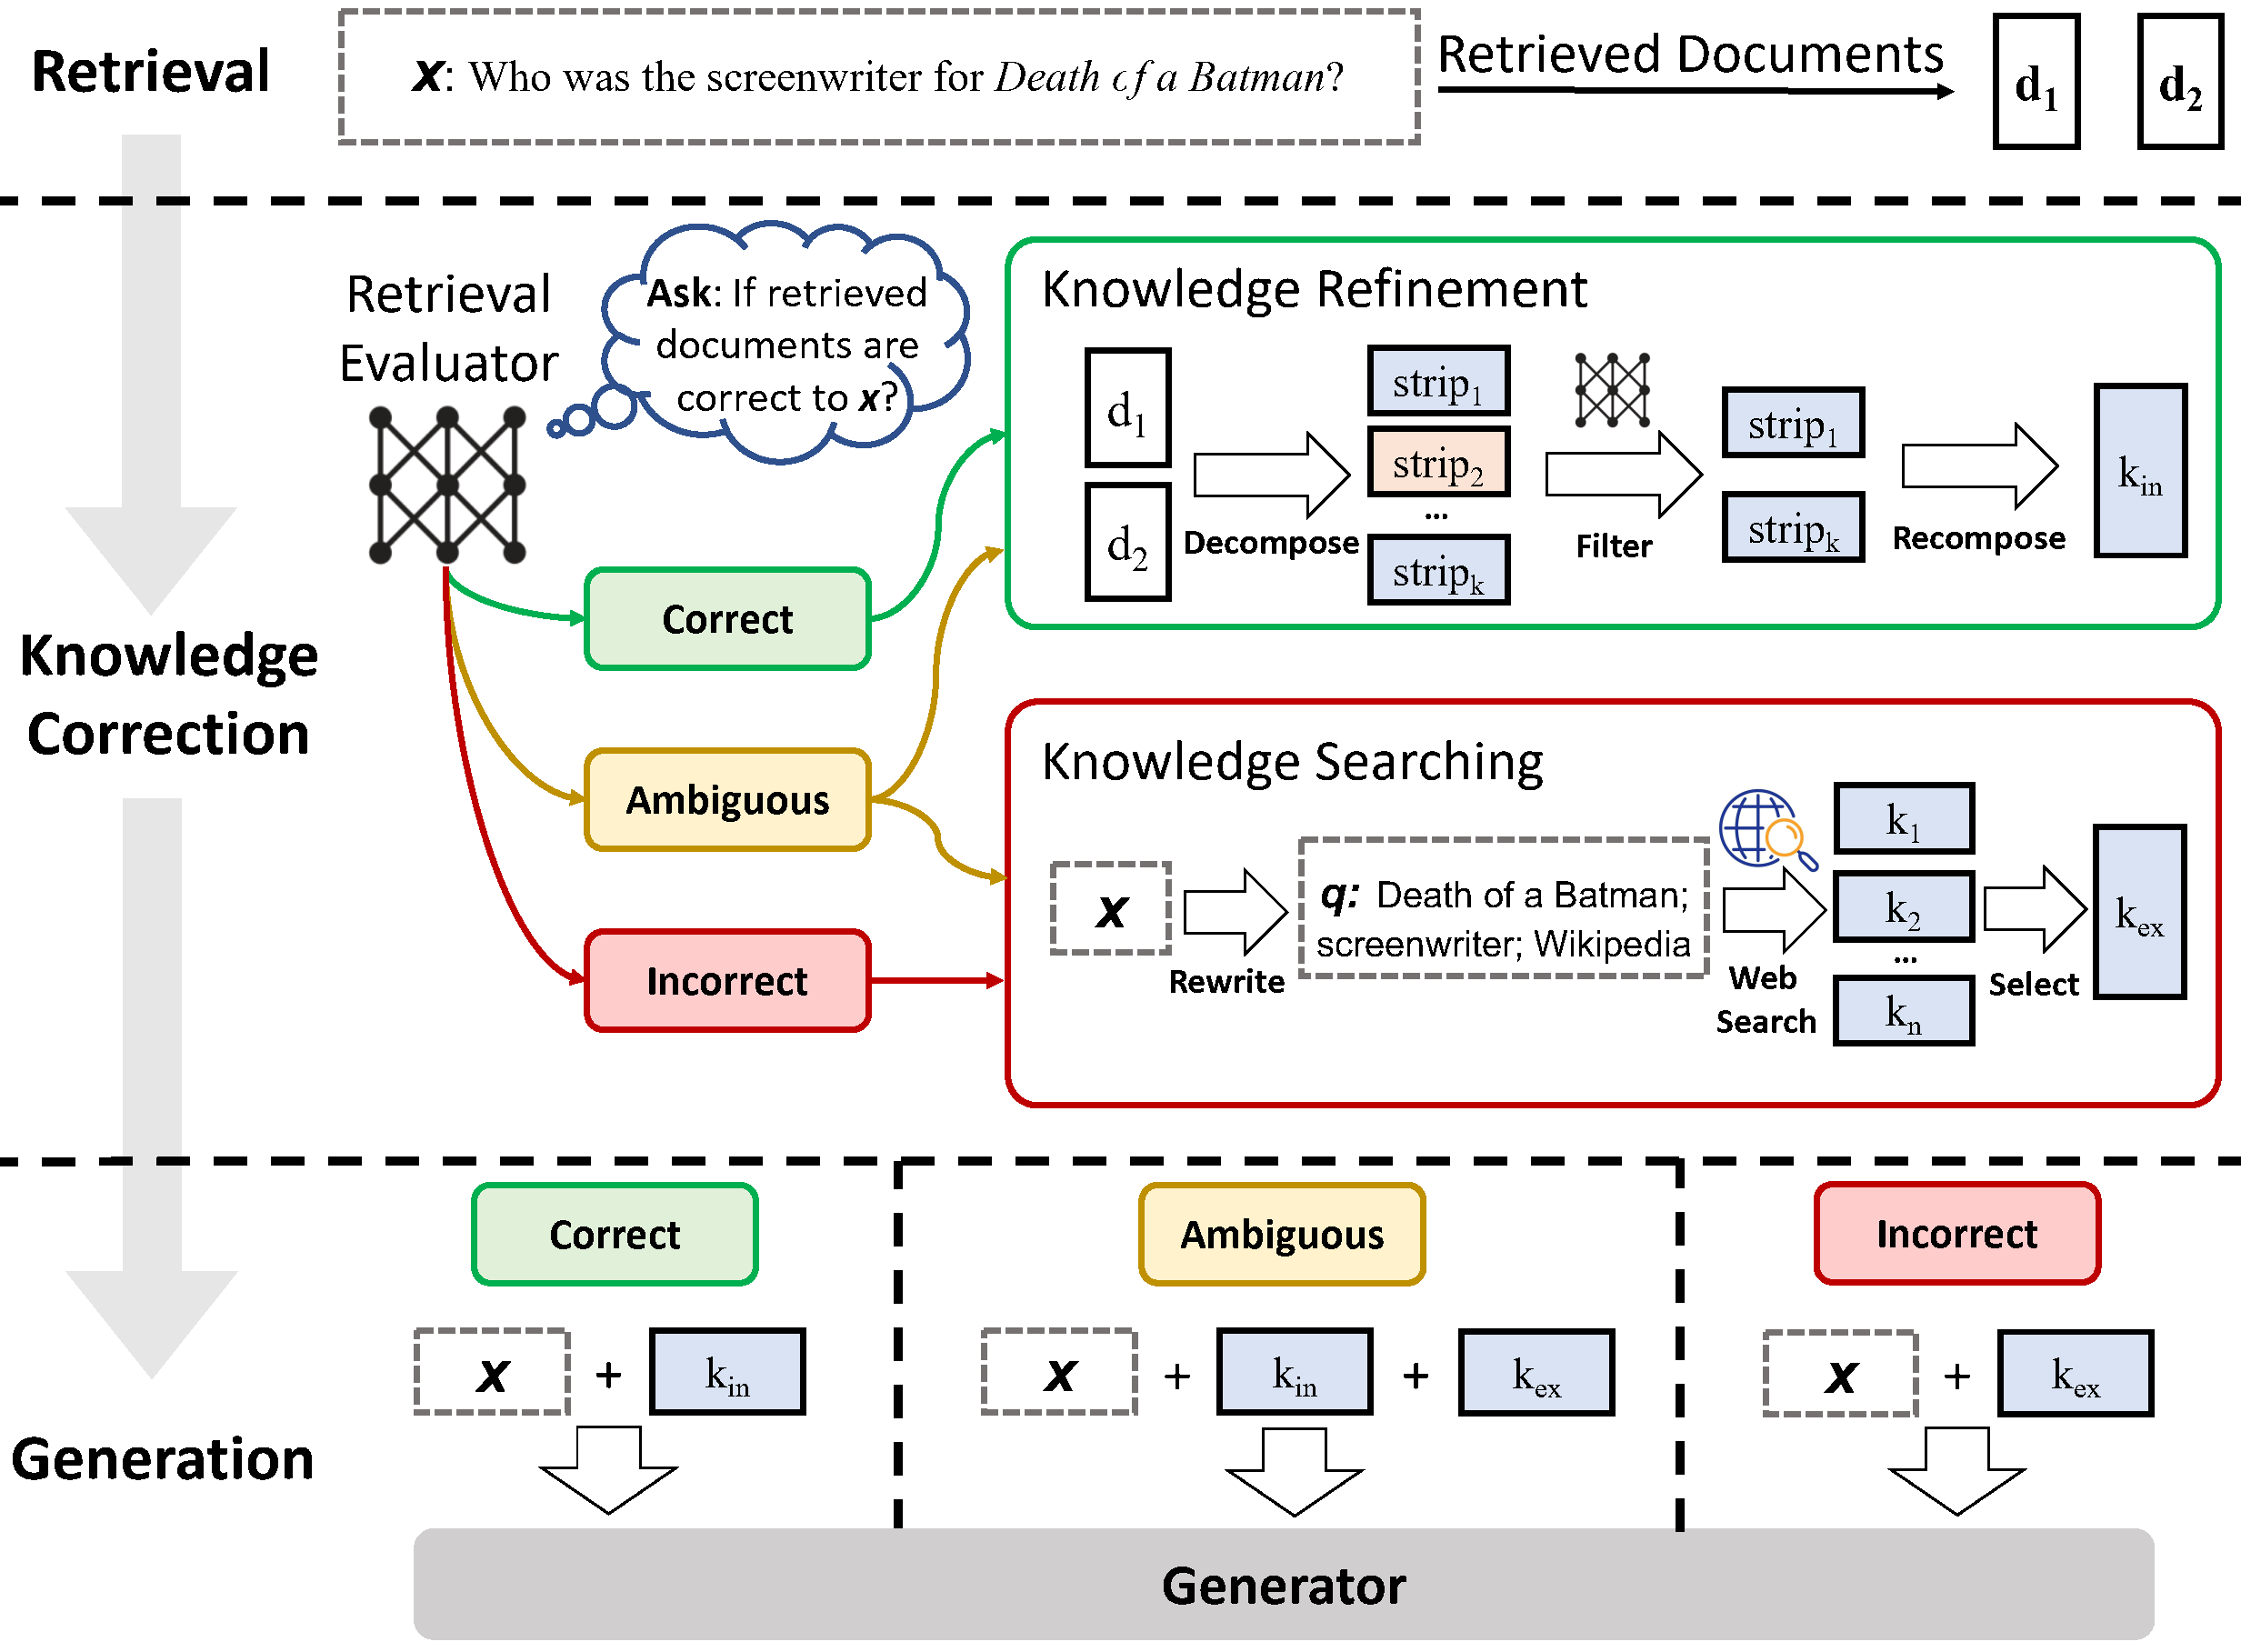
\includegraphics[width=\textwidth]{../images/crag_architecture.png}
\caption{Corrective RAG (CRAG) Workflow. Note that immediately after the User Query, we often perform \textbf{Query Translation using an SLM} before retrieving documents.}
\end{figure}

\section{Hypothetical Document Embeddings (HyDE)}

\begin{figure}[h!]
\centering
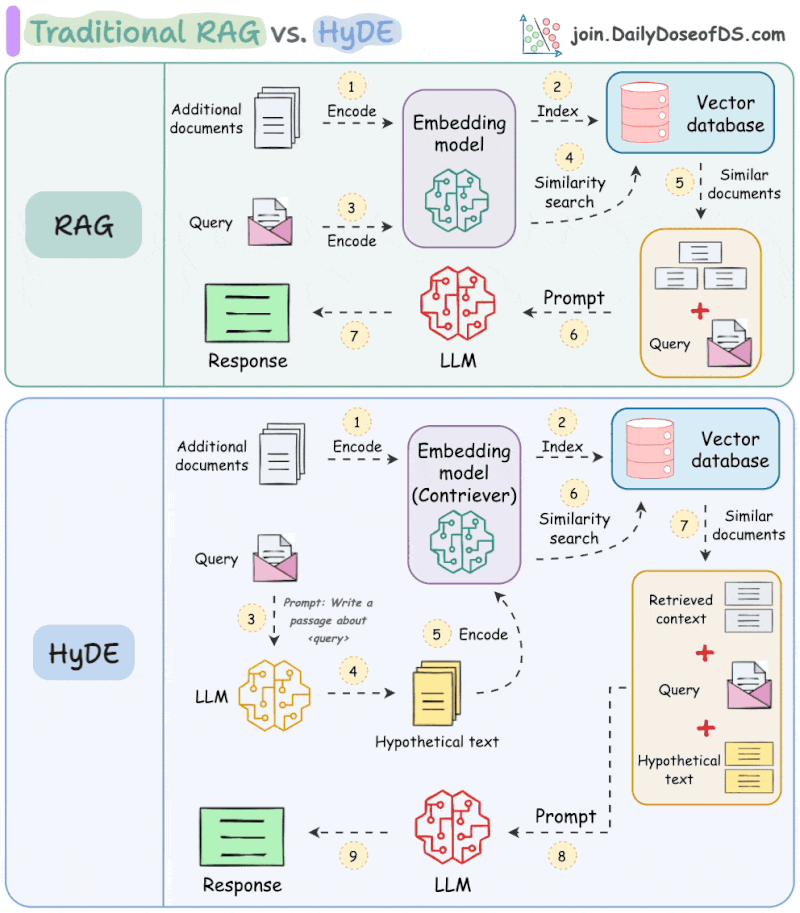
\includegraphics[width=\textwidth]{../images/rag_vs_hyde.png}
\caption{Traditional RAG vs. HyDE Workflow Comparison}
\end{figure}

When a user asks a short question (e.g., "How long to remove wisdom tooth?"), semantic search often fails because a short question does not structurally match a long, detailed medical document. \textbf{HyDE (Hypothetical Document Embeddings)} solves this by searching \textit{document-to-document}.

Instead of embedding the raw query, HyDE passes the query to an LLM to generate a "fake" hypothetical answer. Even if the LLM hallucinates facts, this fake document perfectly captures the vocabulary, tone, and structure of the expected result. We then embed this hypothetical document to search the Vector DB. This drastically improves retrieval accuracy.

\begin{figure}[h!]
\centering
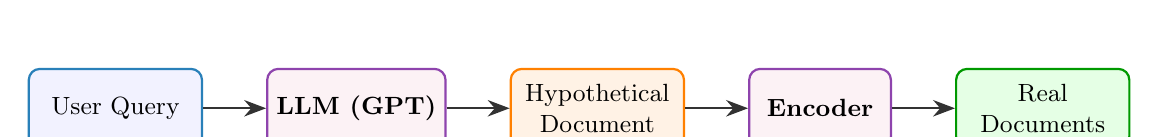
\begin{tikzpicture}[
    node distance=1cm and 0.8cm,
    box/.style={rectangle, draw=primary, fill=blue!5, thick, minimum width=2.2cm, minimum height=1cm, align=center, rounded corners, font=\small},
    model/.style={rectangle, draw=secondary, fill=purple!5, thick, minimum width=1.8cm, minimum height=1cm, align=center, rounded corners, font=\small\bfseries},
    arrow/.style={-{Stealth[scale=1.2]}, thick, draw=darkgray}
]

% Nodes
\node[box] (query) {User Query};
\node[model, right=of query] (gpt) {LLM (GPT)};
\node[box, right=of gpt, fill=orange!10, draw=orange] (hypo) {Hypothetical\\Document};
\node[model, right=of hypo] (encoder) {Encoder};
\node[box, right=of encoder, fill=green!10, draw=green!60!black] (results) {Real\\Documents};

% Arrows
\draw[arrow] (query) -- (gpt);
\draw[arrow] (gpt) -- (hypo);
\draw[arrow] (hypo) -- (encoder);
\draw[arrow] (encoder) -- (results);

\end{tikzpicture}
\caption{Hypothetical Document Embeddings (HyDE) Architecture}
\end{figure}

\chapter{Agentic Patterns \& Orchestration}
AI Agents are LLMs equipped with "hands and legs"---tools (functions) they can execute to interact with the external world (e.g., searching the web, querying a database, firing an email).

\section{The Shift: LangChain to Native Agent SDKs}
Early agent orchestration was heavily node-based and overly abstracted (e.g., LangChain and LangGraph). While excellent for prototyping, they proved difficult to scale and debug. The industry standard has shifted to native \textbf{Agent SDKs} (Vercel AI SDK, Anthropic SDK, OpenAI Swarm).
\begin{itemize}
    \item \textbf{Function Calling (bind\_tools):} The LLM is provided a JSON schema defining available tools. If the LLM decides a tool is needed, it responds with a tool call intent and the necessary arguments.
    \item \textbf{Zod Validation:} Tool arguments generated by the LLM are validated against strict Zod schemas to ensure type-safety before execution.
\end{itemize}

\section{The While-Loop Orchestrator}
Modern agents operate in a ReAct (Reason + Act) while-loop. 
\begin{enumerate}
    \item Evaluate the user prompt and conversation history.
    \item Decide to either output a final text answer or call a tool.
    \item If a tool is called, pause generation, execute the tool locally on the server.
    \item Append the tool's execution result back to the context array.
    \item Repeat the loop until the LLM decides no more tools are needed.
\end{enumerate}

\begin{warningbox}[Max-Turn Limits]
Agents can get stuck in infinite loops if a tool continuously fails or returns unexpected data. A hard limit on execution turns (e.g., max\_turns = 5) is mandatory in production to prevent massive billing spikes.
\end{warningbox}

\section{Observability and Tracing}
Because agents are autonomous, standard HTTP logging is insufficient. Tools like \textbf{LangSmith} or \textbf{Datadog} are critical for tracing the exact steps, tool inputs/outputs, latency, and token costs incurred during an agent's execution loop.

\section{The Manager \& Handoff Patterns}
For complex workflows, a single agent shouldn't possess every tool (which dilutes focus and eats context). 
\begin{itemize}
    \item \textbf{Manager Agent:} A supervisor that evaluates the query and routes it to specialized sub-agents.
    \item \textbf{Handoffs:} An agent can yield its execution context to another agent seamlessly (e.g., the Triage Agent hands off the conversation to the Billing Agent).
\end{itemize}

\chapter[Memory Systems \& Knowledge Graphs]{Memory Systems \&\\Knowledge Graphs}

\section{Tiered Memory Architectures}
Since LLMs are stateless, "memory" is simply the data injected into the system prompt before the call. To ensure agents remember users across sessions without exceeding context windows, memory is tiered:
\begin{itemize}
    \item \textbf{Transient / Short-Term Memory:} The immediate conversation history of the current active session. Typically cached in \textbf{Redis} for extremely fast read/write access.
    \item \textbf{Factual / Episodic Long-Term Memory:} An observation loop runs asynchronously, summarizing the conversation to extract core facts ("User prefers Python"). These facts are stored persistently in a database (like \textbf{Mem0} or \textbf{Qdrant}) and retrieved via semantic search when the user starts a new session weeks later.
\end{itemize}

\section{Knowledge Graphs (Graph RAG)}
While Vector DBs are excellent for unstructured semantic similarity, they lack relational awareness.
\begin{itemize}
    \item \textbf{Relational Memory:} We use Graph Databases like \textbf{Neo4j} to represent entities as nodes and relationships as edges.
    \item \textbf{Use Case:} In Legal Tech or complex HR systems, knowing "Employee A reports to Manager B who owns Project C" requires multi-hop graph traversal (using Cypher queries). Hybrid RAG systems query both a Vector DB (for document text) and a Graph DB (for explicit relationships).
\end{itemize}

\chapter[Advanced Interactions: Voice \& MCP]{Advanced Interactions:\\Voice \& MCP}

\section{Voice Agents \& WebRTC}
Modern voice-to-voice agents require ultra-low latency, making standard HTTP request-response cycles obsolete. They utilize \textbf{WebRTC} (via platforms like LiveKit) to stream audio packets bidirectionally in real-time.

\begin{warningbox}[Security Anti-Pattern: Hardcoded Keys]
Never expose OpenAI or Anthropic API keys in client-side code. Doing so allows anyone inspecting your frontend network calls to steal your keys and run up your bill.
\end{warningbox}
\textbf{The Remote Proxy Pattern:} Instead of direct client-to-LLM communication using root keys, the client requests an \textbf{Ephemeral Key/Token} from your backend. The backend securely negotiates a short-lived, permission-scoped token from the AI provider, which the frontend uses to establish the direct WebRTC connection.

\section{Model Context Protocol (MCP)}
Created by Anthropic, MCP is an open standardization protocol to connect AI models with external tools and data sources securely.
\begin{itemize}
    \item \textbf{Standardization:} Defines a standard JSON schema for tools. If a tool is written as an MCP Server, any compatible MCP Client (Claude Desktop, Cursor, Gemini) can interface with it effortlessly.
    \item \textbf{Architecture Shift:} Early MCP versions were stateful (holding persistent transport connections via STDIO). The protocol is migrating to a \textbf{stateless} architecture (HTTP/SSE) to solve massive scaling bottlenecks.
\end{itemize}

\chapter[Deployment, Scaling, \& Architecture]{Deployment, Scaling,\\\& Architecture}
Deploying a Generative AI application involves traditional backend scaling combined with AI-specific rate-limiting bottlenecks.

\section{Rate Limiting \& Queues}
When scaling an application to thousands of concurrent users, your backend servers might handle the load easily, but your third-party AI provider (OpenAI/Anthropic) will strictly enforce API Rate Limits (e.g., Max 500 requests per minute), throwing \texttt{429 Too Many Requests} errors and crashing your system.
\begin{bestpractice}[Queue-Based Rate Limiting]
Never make direct synchronous LLM calls in high-traffic APIs. Decouple client requests using a Message Queue (\textbf{AWS SQS}, \textbf{RabbitMQ}, or \textbf{BullMQ}). A pool of backend workers consumes the queue at a throttled rate strictly lower than your API limits, ensuring stability.
\end{bestpractice}

\section{AWS Deployment \& Security}
\begin{itemize}
    \item \textbf{EC2 \& Security Groups:} EC2 instances are protected by Security Groups (firewalls). You must explicitly configure Inbound rules (e.g., port 80 for HTTP, port 22 for SSH). Never allow port 22 to the public; restrict it solely to your office/VPN IP address.
    \item \textbf{Load Balancers:} EC2 instances should remain in private subnets. Only a public Load Balancer should be exposed to the internet, proxying requests securely to your EC2 instances.
\end{itemize}

\section{Zero-Downtime Deployments}
When shipping new agent prompts or backend logic, downtime means lost business. Modern DevOps practices include:
\begin{itemize}
    \item \textbf{Blue-Green Deployment:} Spin up a new identical environment (Green) with the updated code. Route traffic to Green. If stable, terminate the old environment (Blue). If it fails, routing back to Blue is instantaneous.
    \item \textbf{Rolling Updates:} Gradually replace instances of the old version with the new version one by one behind the AWS Load Balancer.
\end{itemize}

\chapter[Study Material: Interview \& Viva Prep]{Study Material:\\Interview \& Viva Prep}
\section{Multiple Choice Questions (MCQs)}

\begin{enumerate}
    \item \textbf{What is the primary function of the Transformer architecture in an LLM?} \\
    A) Image classification \\
    B) Predicting the next token \\
    C) Connecting to relational databases \\
    D) Routing network traffic \\
    \textit{Answer: B}

    \item \textbf{Why are Vector Databases used in RAG systems instead of traditional relational databases?} \\
    A) They support SQL queries natively. \\
    B) They are optimized for retrieving semantically similar high-dimensional embeddings. \\
    C) They run directly inside the LLM context window. \\
    D) They do not require chunking. \\
    \textit{Answer: B}

    \item \textbf{What is the core difference between a Vector DB and a Graph DB in the context of RAG?} \\
    A) Vector DBs store relationships; Graph DBs store embeddings. \\
    B) Vector DBs store unstructured semantic embeddings; Graph DBs excel at mapping explicit entity relationships. \\
    C) Graph DBs are much faster for cosine similarity searches. \\
    D) There is no difference; they are interchangeable. \\
    \textit{Answer: B}

    \item \textbf{When deploying a high-traffic GenAI application, how should third-party LLM rate limits be handled?} \\
    A) By increasing the RAM on the backend server. \\
    B) By running the LLM locally. \\
    C) By using a message queue (like AWS SQS) to throttle outbound requests. \\
    D) By using a Blue-Green deployment strategy. \\
    \textit{Answer: C}

    \item \textbf{What is the "Manager Pattern" in Agent orchestration?} \\
    A) The user manually approves every tool call. \\
    B) A central supervisor agent evaluates the prompt and routes it to specialized sub-agents. \\
    C) An orchestrator that restarts the server if memory overflows. \\
    D) A legacy system replaced by vector indexing. \\
    \textit{Answer: B}

    \item \textbf{Why is 'Chunking' necessary in RAG architectures?} \\
    A) Vector DBs only accept 10 words at a time. \\
    B) LLMs have strict context window limitations; feeding an entire enterprise document at once will fail or cause severe attention dilution. \\
    C) To improve the UI rendering speed. \\
    D) To encrypt the data before processing. \\
    \textit{Answer: B}

    \item \textbf{Which deployment strategy involves maintaining two identical production environments to ensure zero downtime?} \\
    A) Containerization \\
    B) Rolling Updates \\
    C) Blue-Green Deployment \\
    D) Stateful Proxies \\
    \textit{Answer: C}
\end{enumerate}

\section{Viva \& Theory Questions}

\textbf{Q: Explain why LLMs are considered "stateless" and how we build conversational memory.} \\
\textit{Answer:} LLMs do not retain memory of previous interactions. Every API request is treated as entirely isolated. To build memory, the application layer must store the conversation history (e.g., in Redis) and append the entire historical context to every new prompt so the LLM has all the required information to generate an accurate response.

\textbf{Q: Describe the workflow of Corrective RAG (CRAG) / Query Rewriting.} \\
\textit{Answer:} Raw user queries are often ambiguous, filled with pronouns or poorly structured for dense vector retrieval. In query rewriting, we pass the raw query to a smaller, faster model (SLM) to rephrase it into a standalone, explicit, highly-indexable search query before running the semantic search against the vector database.

\textbf{Q: Why are modern Agent SDKs migrating towards a while-loop architecture with Max-Turn limits?} \\
\textit{Answer:} Agents autonomously decide to call tools based on user prompts. A ReAct while-loop allows the agent to continuously call a tool, ingest the JSON response, evaluate the new state, and call more tools if necessary. Max-turn limits are crucial to prevent the agent from entering an infinite loop (e.g., a tool repeatedly failing), which would cause massive API token billing spikes.

\textbf{Q: You are building a WebRTC Voice Agent. Why is it a critical security vulnerability to embed the API key in the frontend code, and how do you solve it?} \\
\textit{Answer:} Embedding keys in the frontend exposes them to the client; a malicious user can inspect network traffic, steal the key, and rack up thousands of dollars in usage. The solution is the \textbf{Remote Proxy Pattern using Ephemeral Tokens}. The frontend requests a temporary token from your secure backend. The backend negotiates this with the AI provider, and the frontend uses the ephemeral token to establish a direct WebRTC connection.

\textbf{Q: Explain the difference between Blue-Green Deployments and Rolling Updates.} \\
\textit{Answer:} In a \textbf{Blue-Green Deployment}, you spin up an entirely new environment (Green) alongside the existing one (Blue). Traffic is switched instantly to Green; if successful, Blue is terminated. If it fails, traffic is instantly reverted. In \textbf{Rolling Updates}, new instances progressively replace older instances one by one behind a load balancer, ensuring zero downtime but meaning users might momentarily hit different versions of the application concurrently.

\textbf{Q: How does the Model Context Protocol (MCP) address tool compatibility across different LLMs?} \\
\textit{Answer:} Prior to MCP, every AI framework had a proprietary way of defining tools. MCP provides an open, standardized protocol (JSON schema) for tools. If a tool is written following the MCP standard, any compatible LLM (OpenAI, Claude, Gemini) can discover and execute it without custom integration logic.

\textbf{Q: Explain the difference between Cross-Encoder re-ranking and standard Bi-Encoder semantic search.} \\
\textit{Answer:} A Bi-Encoder (standard vector DB search) embeds the query and documents separately ahead of time, comparing them quickly using cosine similarity. It is fast but lacks deep interaction. A Cross-Encoder takes both the query and the retrieved document simultaneously, passing them together through the transformer layers. It provides highly accurate relevance scoring but is computationally expensive, which is why it is only used as a final re-ranking step on a small subset (e.g., Top-20) of retrieved chunks.

\end{document}
